\label{mapeamento}

Apesar de ser um tema de crescente interesse, tanto 
de pesquisa quanto de aplicação na indústria, a literatura 
não apresenta uma consolidação das principais contribuições 
relacionadas à modernização de sistemas legados. Ou seja, com o 
intuito de descrever adequadamente cenários reais de modernização 
em uma instituição específica, identificou-se  a necessidade 
prévia da condução de \acrfull{MS} para 
caracterizar a modernização de sistemas legados no 
contexto da manutenção de software---uma vez que 
um \acrshort{MS} pode ser conduzido 
para identificar e agregar resultados relevantes 
de estudos sobre determinado tema, ao responder 
questões de pesquisa em particular~\cite{kitchenham:2004,Petersen:2008}. 
Neste capítulo, apresenta-se os resultados da condu\c c\~{a}o de 
um \acrshort{MS} na \'{a}rea de moderniza\c c\~{a}o de software.

\section{Método de Pesquisa}

A condução de mapeamentos sistemáticos na área de 
Engenharia de Software tem se tornado uma prática 
consolidada que envolve um conjunto bem definido 
de atividades~\cite{Petersen:2008}. Esta seção descreve 
o protocolo de estudo usado, 
de acordo com as recomendações já propostas para a 
condução desse tipo de estudo. 

Um protocolo de estudo é um plano com os procedimentos básicos de 
estudos que devem ser utilizados no MS, de acordo com~\cite{Petersen:2008}. 
Dessa forma, seu  uso favorece que o mapeamento 
possa ser reproduzido por outros pesquisadores, 
sem os problemas do viés de publicação 
mencionados em~\cite{kitchenham:2004}. A Figura~\ref{fig:protocolo_pesquisa_ms} 
mostra o protocolo da pesquisa. O restante dessa seção contém as questões de pesquisa, 
a estratégia de busca e os critérios de inclusão e 
exclusão de publicações usados neste mapeamento.


\begin{figure}
\centering
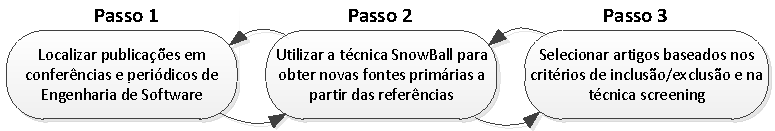
\includegraphics[scale=1.2]{img/mapeamento/protocolo_pesquisa_ms.pdf}
\caption{Protocolo de pesquisa do mapeamento sistemático.}
\label{fig:protocolo_pesquisa_ms}
\end{figure}


\subsection{Questões de Pesquisa (QP)}

As questões de pesquisa foram elaboradas 
de acordo com a motivação deste estudo, 
que visa caracterizar a modernização dos sistemas legados 
no contexto da manutenção de software, ao identificar 
as principais contribuições e estudos na literatura sobre este tema. 
São elas:

\begin{enumerate}[(QP1)]
\item O que caracteriza a modernização dos sistemas legados de 
acordo com a literatura existente? Quais outros termos estão relacionados 
com modernização?

\item Quais processos, técnicas ou ferramentas têm sido sugeridos 
na literatura para suportar as atividades de modernização 
dos sistemas legados?

\item Quais as razões que levam as organizações a 
modernizarem os seus sistemas legados?

\end{enumerate}

\subsection{Estrat\'{e}gia de Busca}

A estratégia de busca consistiu 
na pesquisa manual de publicações disponíveis em conferências 
e periódicos da área de Engenharia de Software. 
Tal estratégia, referenciada em~\cite{kitchenham:2004}, foi adotada 
por entender que seria possível obter artigos de maior relevância 
face ao uso de \textit{strings} de busca, uma vez que os termos 
utilizados para referir a modernização ou evolução de sistemas 
são bem amplos. 

Com isso, a busca foi organizada para ser executada em três etapas. 
Uma lista com as fontes de pesquisa foi selecionada para cada etapa de 
maneira empírica. Essa estratégia foi complementada pela 
técnica ``snowball''~\cite{kitchenham:2004}, 
que objetiva obter novas fontes de pesquisa primárias analisando 
as refer\^{e}ncias dos artigos encontrados. 
As fontes de pesquisa selecionadas foram:

\begin{enumerate}[(a)]

\item Fontes de pesquisa da etapa 1
  \begin{itemize}
   \item{ICSE -- International Conference on Software Engineering;}
   \item{TSE -- Transactions on Software Engineering;}
   \item{SPE -- Software: Practice and Experience;}
   \item{IEEE Software.} 
  \end{itemize}

\item Fontes de pesquisa da etapa 2

  \begin{itemize}
   \item{ICSM -- International Conference on Software Maintenance;}
   \item{WCRE -- Working Conference on Reverse Engineering;}
   \item{CSMR -- Software Evolution Week.} 
  \end{itemize}

\item Fontes de pesquisa da etapa 3

  \begin{itemize}
   \item{ACM Digital Library;}
   \item{IEEE Xplore;}
   \item{SpringerLink;}
   \item{SEI Digital Library;} 
   \item{Science Direct.}
  \end{itemize}

\end{enumerate}

\subsection{Critérios de Inclusão e Exclusão}

A fim de selecionar os estudos primários mais relevantes, restrições de inclusão e exclusão foram estipuladas. 
Para o critério de inclusão, somente as publicações que faziam alusão ao tema abordado no título ou no \textit{abstract} 
cuja data de publicação estivesse compreendido entre 1995 e 2015. 
Este intervalo foi definido para obter o maior número possível de publicações relevantes. 
Para o critério de exclusão, fontes que contribuem com algum resultado (positivo ou negativo), 
que tenham mais de 20 citações e pelo menos 4 páginas.

\subsection{Seleção das Publicações}

A seleção das publicações iniciou com a pesquisa manual nas fontes de pesquisa primárias selecionadas anteriormente, 
observando o protocolo de pesquisa. Com isso, foi gerada uma lista inicial com 59 publicações. Posteriormente, essa lista passou 
para 44 com as técnicas de \textit{screening} sugeridas por~\cite{Petersen:2008} que descartou algumas publicações não 
enquadradas nos critérios do protocolo. A tabela \ref{table:artigos} exibe a lista de publicações selecionadas para análise.

\subsection{Extração de Dados e Análise}

Como pode ser visto na Figura~\ref{fig:grafico_distribuicao}, no gráfico de distribuição à esquerda, 
o \acrfull{IEEE} foi a fonte de pesquisa que retornou 
a maior parcela dos estudos primários com 63.64\%, seguido do Science Direct com 11.36\% e do SEI Digital Library com 9.09\%. 
Supõem-se que é porque o \acrshort{IEEE} possui o maior número de conferências e publicações na área de Engenharia de Software e 
também porque indexam publicações de outras bibliotecas. No gráfico de distribuição à direita, pode-se visualizar 
as principais conferências e jornais que publicaram sobre o tema, destacando-se 
a \acrfull{CSMR} com 21.43\%, e o \acrfull{SEI} com 14.29\%. Todas as demais conferências e jornais possuem 7.14\% de publicações cada uma. 

\begin{figure}
\centering
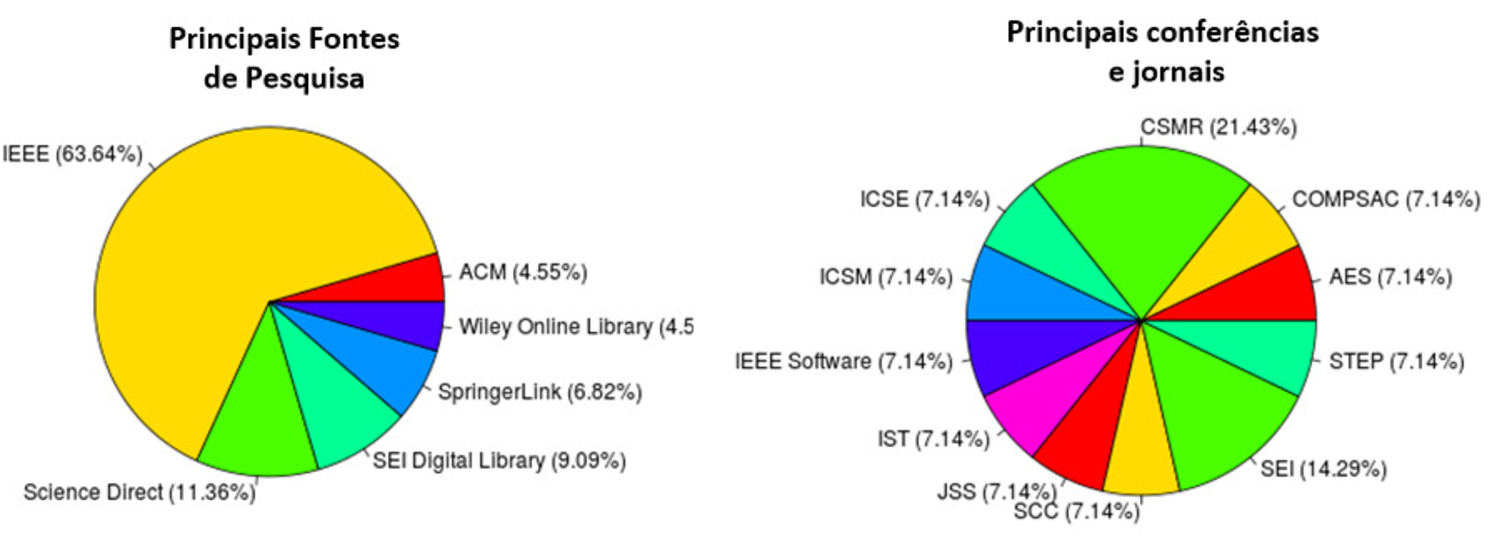
\includegraphics[scale=0.64]{img/mapeamento/grafico_distribuicao.pdf}
\caption{Distribuição das publicações por fontes de pesquisa.}
\label{fig:grafico_distribuicao}
\end{figure}


%% ATENÇÃO: Gerado automaticamente com o programa bibliografia/papers.py
%% Para atualizar: python3.4 papers.py

\makeatletter
    \newcommand{\thickhline}{%
        \noalign {\ifnum 0=`}\fi \hrule height 1pt
        \futurelet \reserved@a \@xhline
    }
    \newcolumntype{"}{@{\vrule width 1pt}}
    \makeatother


\begin{table*}[htbp]
\scalefont{0.72}
\caption {Lista das publicações selecionadas para análise.} \label{table:artigos}
\centering % centering table

\newcolumntype{L}[1]{>{\raggedright\let\newline\\\arraybackslash\hspace{0pt}}p{#1}}
\newcolumntype{C}[1]{>{\centering\let\newline\\\arraybackslash\hspace{0pt}}m{#1}}
\newcolumntype{R}[1]{>{\raggedleft\let\newline\\\arraybackslash\hspace{0pt}}m{#1}}

\definecolor{Gray}{gray}{0.85}
\definecolor{LightCyan}{rgb}{0.88,1,1}

\setlength{\extrarowheight}{0.5pt}


\begin{tabular}{"| L{4.98cm} | L{4.98cm} | L{4.98cm} |"}


\thickhline%\toprule

[1] Bennett et al. Software
maintenance and evolution: a roadmap. ICSE 2000.
&
[2] Erlikh et al. Leveraging legacy system
dollars for e-business. IT professional 2000.
&
[3] Bisbal et al. Legacy information systems:
Issues and directions. IEEE Software 1999.

\\ \hline

[4] Bennett et al. Legacy systems: coping with success. IEEE 1995.
&
[5] Sneed et al. Integrating legacy software into a service oriented architecture. CSMR 2006.
&
[6] Lewis et al. Service-oriented migration and reuse technique (smart). IEEE 2005.
\\ \hline

[7] Canfora et al. A wrapping approach for migrating legacy system interactive functionalities to service oriented architectures. JSS 2008.
&
[8] Zhang et al. Incubating services in legacy systems for architectural migration. IEEE 2004.
&
[9] Canfora et al. Migrating interactive legacy systems to web services. CSMR 2006.
\\ \hline

[10] Bianchi et al. Iterative reengineering of legacy systems. IEEE Transactions 2003.
&
[11] Canfora et al. Decomposing legacy programs: A first step towards migrating to client–server platforms. JSS 2000.
&
[12] Weiderman et al. Approaches to Legacy System Evolution. SEI 1997.
\\ \hline

[13] Wu et al. The butterfly methodology: A gateway-free approach for migrating legacy information systems. IEEE 1997.
&
[14] Sneed et al. Encapsulation of legacy software: A technique for reusing legacy software components. ASE 2000.
&
[15] Comella-Dorda et al. A survey of legacy system modernization approaches. SEI 2000.
\\ \hline

[16] Ransom et al. A method for assessing legacy systems for evolution. SMR 1998.
&
[17] Fleurey et al. Model-driven engineering for software migration in a large industrial context. Springer 2007.
&
[18] Comella-Dorda et al. A survey of black-box modernization approaches for information systems. ICSM 2000.
\\ \hline

[19] Lewis et al. SMART: Analyzing the reuse potential of migrating legacy components to SOA. SEI 2008.
&
[20] Serrano et al. Reengineering legacy systems for distributed environments. JSS 2002.
&
[21] Lucia et al. Developing legacy system migration methods and tools for technology transfer. SPE 2008.
\\ \hline

[22] Lewis et al. Service-oriented architecture and its implications for software maintenance and evolution. FoSM 2008.
&
[23] Moore et al. Migrating legacy user interfaces to the internet: shifting dialogue initiative. WCRE 2000.
&
[24] Warren et al. The renaissance of legacy systems: method support for software-system evolution. Springer 2012.
\\ \hline

[25] Visaggio et al. Value-based decision model for renewal processes in software maintenance. ASE 2000.
&
[26] Weiderman et al. Implications of distributed object technology for reengineering. SEI 1997.
&
[27] Cetin et al. Legacy migration to service-oriented computing with mashups. ICSEA 2007. 
\\ \hline

[28] Colosimo et al. Evaluating legacy system migration technologies through empirical studies. Science Direct 2009.
&
[29] Erradi et al. Evaluation of strategies for integrating legacy applications as services in a service oriented architecture. SCC 2006.
&
[30] Chung et al. Service-oriented software reengineering: SoSR. IEEE 2007.
\\ \hline

[31] Litoiu et al. Migrating to web services: a performance engineering approach. SMR 2004.
&
[32] Liu et al. Reengineering legacy systems with RESTful web service. COMPSAC 2008.
&
[33] O'Brien et al. Supporting migration to services using software architecture reconstruction. IEEE 2005.
\\ \hline

[34] Chiang et al. Wrapping legacy systems for use in heterogeneous computing environments. Science Direct 2001.
&
[35] Smith et al. Migration of legacy assets to service-oriented architecture environments. IEEE 2007.
&
[36] Wu et al. Legacy systems migration-a method and its tool-kit framework. IEEE 1997.
\\ \hline

[37] Bovenzi et al. Enabling legacy system accessibility by web heterogeneous clients. CSMR 2003.
&
[38] Li et al. Migrating legacy information systems to web services architecture. JDM 2007.
&
[39] Zdun et al. Reengineering to the web: A reference architecture. CSMR 2002.
\\ \hline

[40] Cetin et al. A mashup-based strategy for migration to service-oriented computing. IEEE 2007.
&
[41] Zhang et al. A black-box strategy to migrate GUI-based legacy systems to web services. IEEE 2008.
&
[42] Serrano et al. Evolutionary migration of legacy systems to an object-based distributed environment. ICSM 1999.
\\ \hline

[43] Qiao et al. Bridging legacy systems to model driven architecture. COMPSAC 2003.
&
[44] Canfora et al. Software evolution in the era of software services. IEEE 2004.&
\\ \hline
\thickhline%\toprule


\end{tabular}
\end{table*}




\section{Resultados}

Nesta seção, são descritos os resultados do \acrshort{MS} obtidos após o estudo das publicações selecionadas. 
Quanto à resposta a primeira questão, foram analisados os estudos primários 
com o foco na caracterização do tema modernização. Esta faceta foi então combinada para responder a 
segunda questão QP2. Finalmente, na QP3, abordaram-se as razões que levam as organizações a buscarem a 
modernização dos sistemas legados de acordo com a literatura estudada.

\subsection{An\'{a}lise Relacionada à Primeira Questão de Pesquisa}

\begin{enumerate}[(QP1)]

\item O que caracteriza a modernização dos sistemas legados de 
acordo com a literatura existente? Quais outros termos estão relacionados 
com a modernização?

\end{enumerate}

Para responder essa questão, buscou-se caracterizar a modernização dos sistemas 
legados no contexto da manutenção de software. Assim, como pode-se 
verificar em~\cite{S01_bennett2000software, S9_bianchi:2003, S3_Bisbal:1999, S15_Comella-DordaASurvey2000, S2_erlikh:2000}, 
a modernização pode ser caracterizada pela necessidade de evolução dos sistemas para adequá-lo aos requisitos de negócio das organizações, 
seja com novas funcionalidades, correção de erros ou atualizações tecnológicas. Nesse sentido, muitas teorias 
tem sido sugeridas na literatura, como discutido a seguir. 

\textbf{N. Weiderman et al.} introduzem um modelo de ciclo de vida 
para descrever a evolução de um sistema durante a sua vida útil~\cite{S15_Comella-DordaASurvey2000, Seacord:2003, S12_WeidermanApproaches:1997}. 
Neste modelo, existem três fases distintas: manutenção, modernização e substituição. Durante o ciclo de vida de um sistema, pequenas 
modificações são realizadas através das manutenções para satisfazer algum requisito ou corrigir algum erro. As mudanças de maior impacto, 
como requisitos de negócios importantes, mudanças na arquitetura do sistema ou a migração do sistema para outra plataforma são realizadas na fase 
de modernização. Todavia, quando o sistema torna-se muito resistente para evoluir por alguma razão específica, este é substituído. 
Nesse ciclo, as necessidades de negócio da organização são intercaladas com as implementações realizadas para suprir essas necessidades. 
Além de introduzir um modelo de ciclo de vida, Weiderman também propõem distinguir a modernização pelo nível de compreensão requerido para suportar 
os esforços de modernização: \textit{White-box} para compreensão das estruturas internas do sistemas e \textit{Black-box} quando requer somente a compreensão das interfaces externas dos sistemas legados.

\textbf{K. Bennett et al.} propõem um modelo chamado 
\textit{staged model} para descrever o ciclo de vida de um sistema e auxiliar na identificação das principais 
áreas de pesquisa sobre modernização~\cite{S01_bennett2000software}. Este modelo divide-se em 5 etapas: 
\textit{initial development, evolution, servicing, phase-out, close-down}. Aqui, a modernização compreende a fase \textit{evolution} e, 
ao contrário do modelo proposto por Weiderman et al., é considerada uma atividade de manutenção, que pode ser classificada em 
4 classes: adaptativa, quando há alterações no ambiente do software; perfectiva, para novos requerimentos do usuário; corretiva, correção de erros; e preventiva, para 
prevenir problemas futuros. 

\textbf{J. Bisbal et al.} apresentam um modelo de ciclo de vida, onde o foco são as atividades evolutivas ordenadas pelo impacto causado nos 
sistemas~\cite{S3_Bisbal:1999}. Assim, dividem-se em \textit{wrapping}, cujo objetivo é prover uma nova interface para os componentes de um sistema, 
tornando-os mais acessíveis para outros componentes; manutenção, para os pequenos ajustes e correção de erros; a migração, que visa mover o sistema 
legado para um ambiente mais flexível, mantendo os dados e funcionalidades originais; e o redesenvolvimento, que reescreve por completo as aplicações. 

Percebe-se que, embora esses modelos usem termos distintos para referir-se as fases do ciclo de vida dos sistemas, há várias semelhanças. Por exemplo, 
o significado de substituição é o mesmo que redesenvolvimento e o significado de migração é o mesmo que modernização. No entanto, 
a fase \textit{wrapping} descrita por Bisbal et al. é uma técnica de modernização \textit{Black-box} em Weiderman.

Prosseguindo com esta análise, tendo em vista à diversidade de termos para referir-se as abordagens de modernização, 
para responder as demais questões de pesquisa, optou-se pelo modelo proposto por Weiderman et al.. Sendo assim, segue um breve resumo de cada 
fase neste modelo evolutivo:

\begin{description}

\item[Manutenção] é a primeira fase do ciclo de vida de um sistema. Ela inicia tão logo o sistema entra em produção, 
sendo considerado um processo iterativo e incremental, através do qual, pequenas modificações são aplicadas ao sistema, 
de maneira pontual e localizada~\cite{S01_bennett2000software, S12_WeidermanApproaches:1997}. No entanto, como salienta~\cite{Seacord:2003}, 
essas modificações atendem as necessidades das organizações apenas por um determinado período, deteriorando-se posteriormente.

\item[Modernização] ocorre quando a manutenção não é suficiente para manter o sistema atualizado e alinhado aos objetivos de negócios. 
Segundo~\cite{S01_bennett2000software, S3_Bisbal:1999, S12_WeidermanApproaches:1997}, compreendem alterações maiores, como por exemplo, a implementação de um requisito importante, 
mudanças na arquitetura ou migração do sistema para uma nova plataforma. Assim, como observado em~\cite{S01_bennett2000software}, a modernização é mais pervasiva que a manutenção, 
sendo um dos principais aspectos que os diferenciam. Por fim, conforme salienta~\cite{Seacord:2003}, a modernização deve preservar as funcionalidades e os dados do sistema, caso contrário, 
representaria uma substituição. 

\item[Substituição] fase também conhecida como \textit{Big Bang} ou \textit{Cold Turkey}~\cite{Seacord:2003}, normalmente é utilizada quando o sistema 
legado torna-se muito resistente e inflexível para ser modernizado, não há documentação ou o custo de manutenção não compensa mais~\cite{S01_bennett2000software, S3_Bisbal:1999, S12_WeidermanApproaches:1997}.

\end{description}

Com este breve resumo das características de cada fase do ciclo de vida de um sistema, finaliza-se a questão QP1 com um \textit{word cloud} 
dos 30 termos mais citados nos \textit{abstracts} das fontes primárias selecionadas. Esses termos podem ser visualizados na 
Figura~\ref{fig:word_cloud}. Note que, sob a perspectiva tecnol\'{o}gica, \'{e} poss\'{i}vel perceber nessa figura um certo grau de 
interesse na computa\c c\~{a}o orientada a servi\c cos. 


\begin{figure}[ht]
\centering
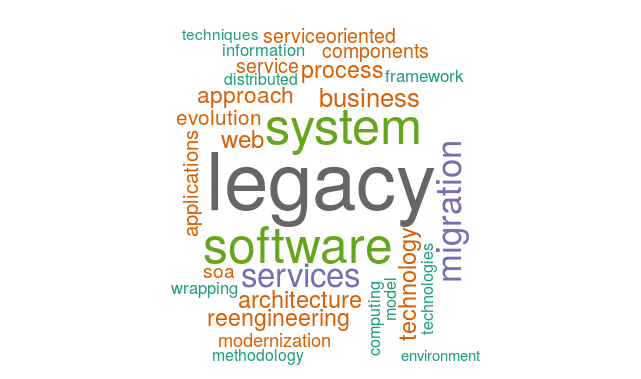
\includegraphics[scale=0.40]{img/mapeamento/word_cloud.png}
\caption{Termos mais citados nos \textit{abstracts} das fontes primárias selecionadas.}
\label{fig:word_cloud}
\end{figure}

\subsection{Análise Relacionada à Segunda Questão de Pesquisa}

Esta questão busca verificar se a abordagem orientada a serviços melhora a qualidade dos produtos de software desenvolvidos no CPD/UnB, a fim de satisfazer as necessidades dos usuários. 
Para isso, faz-se uma análise qualitativa da capacidade de manutenibilidade do novo sistema \acrshort{SAE} a partir da experiência dos participantes do estudo de caso. 

A análise foi realizada em conformidade com a norma de qualidade NBR ISO/IEC 9126-1~\cite{iso2003iec}. Esta norma recomenda que seja definido um \emph{modelo de qualidade} para uma avaliação. Assim, foi definido um modelo de qualidade com base no \emph{modelo de qualidade externa e interna} referido pela norma, como mostra a Figura~\ref{fig:modelo_qualidade}. 


% Modelo de qualidade proposto
%======================================================================================

\begin{figure}[htb]
\centering
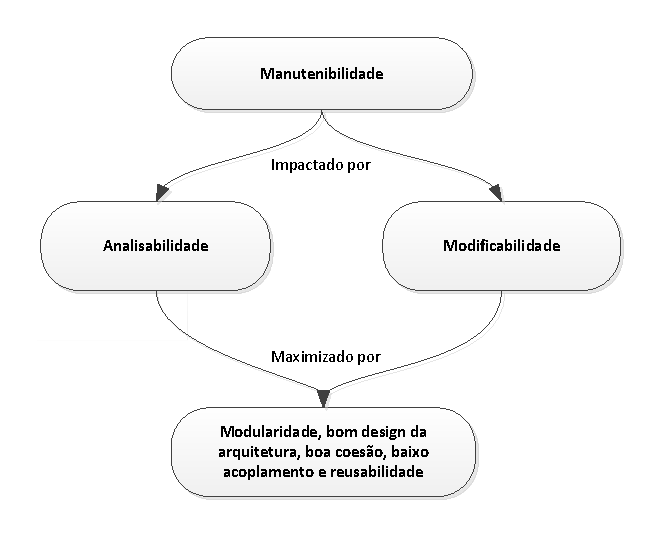
\includegraphics[scale=1]{/img/avaliacao/QP2/modelo_qualidade.pdf}
\caption{Modelo de qualidade proposto para responder a QP2.}
\label{fig:modelo_qualidade}
\end{figure}

O modelo proposto avalia a característica de \emph{manutenibilidade} do
produto de software desenvolvido no estudo de caso (o novo sistema \acrshort{SAE}), 
sendo que foram selecionadas as sub-características da manutenibilidade denominadas
\emph{analisabilidade} e \emph{modificabilidade}, 
as quais servem como uma lista de verificação
de tópicos relacionados com a qualidade avaliada nessa questão. 

A manutenibilidade é uma característica inerente a um produto de software e refere-se a capacidade do mesmo em sofrer correções, melhorias ou adaptações para satisfazerem aos requisitos ou especificações funcionais dos usuários~\cite{iso2003iec, sant2003reuse}. Por definição, a sub-característica analisabilidade compreende a capacidade do produto de software em permitir um diagnóstico das deficiências ou causas de falhas no software, ou a identificação de partes a serem modificadas. Por sua vez, a sub-característica modificabilidade representa a capacidade do produto de software em permitir que uma modificação especificada seja implementada~\cite{iso2003iec}.

É importante salientar, como sugere~\cite{fenton2014software}, que não é possível na prática
medir todas as sub-características internas e externas de um produto
de software, razão pela qual delimitou-se 
nesta investigação as sub-características analisabilidade e modificabilidade
da manutenibilidade, uma vez que o
foco do trabalho de dissertação é propor uma abordagem \acrshort{SOA} 
que seja de fácil manutenção. 

Tradicionalmente, o trabalho de manutenção em um software ocorre após o mesmo entrar em produção e é necessário satisfazer algum requisito ou necessidade que justifique a sua alteração. Para~\cite{S01_bennett2000software}, a manutenção prolonga a vida útil de um software ao mantê-lo atualizado, devendo ser incorporada ao produto de software desde o início de seu desenvolvimento.

Em um primeiro momento, buscou-se verificar a manutenibilidade do sistema \acrshort{SAE}, analisando empiricamente as sub-características analisabilidade e modificabilidade de forma qualitativa. Posteriormente, ao final deste capítulo, será apresentado uma avaliação quantitativa baseada nas métricas propostas por Chidamber \& Kemere~\cite{chidamber1994metrics} para complementar a análise qualitativa, sendo portanto, secundário neste trabalho de dissertação.

De acordo com~\cite{sant2003reuse}, há várias formas de se avaliar a manutenibilidade de um produto de software. Por exemplo, medindo o tempo para aplicar determinada alteração no código fonte ou esforço para diagnosticar determinado problema no software. Também pode-se acompanhar o histórico de modificações de um sistema no repositório de versões desse software. Nesta avaliação, optou-se por mensurar a manutenibilidade por meio da comparação do código fonte do \acrshort{SAE} e outros sistemas da \acrshort{UnB}.

As Figuras~\ref{fig:dependency_diagram_sae_vb},~\ref{fig:dependency_diagram_sae_csharp} 
e~\ref{fig:dependency_diagram_sae_java} mostram três diagramas da arquitetura do \acrshort{SAE} e suas dependências nas versões VB, C\# e Java, respectivamente. Destaca-se que a versão em Java foi desenvolvida durante o estudo de caso com a abordagem proposta neste trabalho de dissertação. Esses diagramas foram produzidos 
utilizando a suíte de ferramentas de análise estática da empresa CodeGear, 
disponível no sítio \url{http://www.codergears.com}. 

Como pode-se observar nos diagramas apresentados, tanto a versão VB quanto a C\# possuem um design monolítico em sua arquitetura. O design monolítico compreende uma das arquiteturas mais comuns e antigas da Engenharia de Software, onde os componentes estão contidos no núcleo do sistema. Nesse \emph{tipo de arquitetura}, como salienta~\cite{clements2002documenting}, a aplicação é composta por vários módulos que são compilados e unidos formando um grande sistema. A maioria dos sistemas em VB e C\# da \acrshort{UnB} segue esta arquitetura, sendo projetados com baixa modularidade e sem qualquer compromisso com o reuso na época em que foram desenvolvidos. 

Segundo o Gestor dos sistemas acadêmicos do CPD/UnB, os principais problemas decorrentes dessa arquitetura, observados nos sistemas legados da \acrshort{UnB}, estão relacionados com a complexidade e o tamanho dos códigos fonte que dificultam a compreensão e a manutenção. Por exemplo, na versão VB do \acrshort{SAE} 
identificou-se um artefato chamado \emph{frmAtzEstSocioEconomico} com aproximadamente 6673 linhas de código. 

Nesse caso, módulos com muitas responsabilidades são difíceis de entender, como é possível presumir, tornando a manutenção muito resistente, passível de erros e comprometendo as propriedades de analisabilidade e modificabilidade. Por conta disso, os desenvolvedores do CPD/UnB, geralmente, evitam alterar os sistemas legados, a não ser quando realmente necessárias.

De modo geral, a única forma de reuso nesses sistemas se dá por meio do acesso ao banco de dados ou através de bibliotecas de funções. Assim, quando necessita-se compartilhar dados ou alguma lógica de negócio, normalmente, criam-se \textit{views} ou \textit{stored procedures} no banco de dados. As bibliotecas de funções contém funções de uso geral e não estão estritamente ligadas as regras de negócios dos sistemas da \acrshort{UnB}. Especificamente, nas aplicações em VB, são muito comuns as regras de negócios estarem na mesma camada onde implementam-se as interfaces com o usuário. Consequentemente, fragmentos de regras de negócios são replicadas em várias telas, dificultando a modificação do software, pois se uma regra mudar, o desenvolvedor precisa revisar o código do sistema para garantir que a lógica foi alterada em todos os locais. 

Por outro lado, até mesmo os sistemas desenvolvidos em Java a partir de 2010
seguem uma arquitetura monolítica com algumas melhorias de design discutidas mais adiante, como 
é o caso do sistema \acrshort{SIGER}, o gerador de relatórios para as aplicações web; o \acrshort{SIEX}, o sistema de informações e extensão; e o \acrshort{SIMAR}, o sistema para gestão das compras de materiais da Universidade. Como curiosidade, o \acrshort{SIMAR} foi migrado parcialmente para Java de acordo com o seu direcionamento estratégico que foi priorizar o módulo de pedidos enquanto que o restante do sistema continuaria funcionando na versão legada. Note que,
sem uma abordagem orientada a serviços, as regras de negócios contidas na versão VB do \acrshort{SIMAR} foram replicadas na versão em Java e, atualmente, a versão Java já contém funcionalidades
não presentes na versão legada, resultado da evolução natural do sistema para atender os 
requisitos dos usuários.


Os sistemas em C\# e Java da \acrshort{UnB} utilizam também uma arquitetura em três camadas para separar a interface com o usuário, o domínio de negócio e a camada de persistência das aplicações. De acordo com a literatura, a arquitetura em camadas auxilia na separação de conceitos e pode trazer ganhos na facilidade de compreensão e na manutenção dos sistemas~\cite{clements2002documenting}. Contudo, o design das aplicações da \acrshort{UnB} continuaram monolíticas, não sendo possível conversarem entre si, a não ser pelo banco de dados. Mesmo com a introdução de bibliotecas compartilhadas para as regras de negócios (introduzido pelo CPD em 2013), ainda era necessário recompilar os sistemas e muitas vezes o desenvolvedor não conseguia reutilizar as bibliotecas devido as dependências circulares existentes. A impossibilidade de reutilizar as regras de negócios de maneira fácil acabou gerando um grande problema para o CPD: a duplicação das classes de negócios entre os sistemas. Assim, os códigos das classes de negócios foram sendo aos poucos replicados entre os sistemas, conforme a necessidade do desenvolvedor. A Figura \ref{fig:duplicidade_usuario_negocio} ilustra esse problema com a classe \emph{UsuarioNegocio} que está replicada em vários sistemas Java. Outro ponto colateral dessas redundâncias, é que muitas classes após serem replicadas, sofrem modificações e começam a evoluir separadamente.

\begin{figure}[ht]
\centering
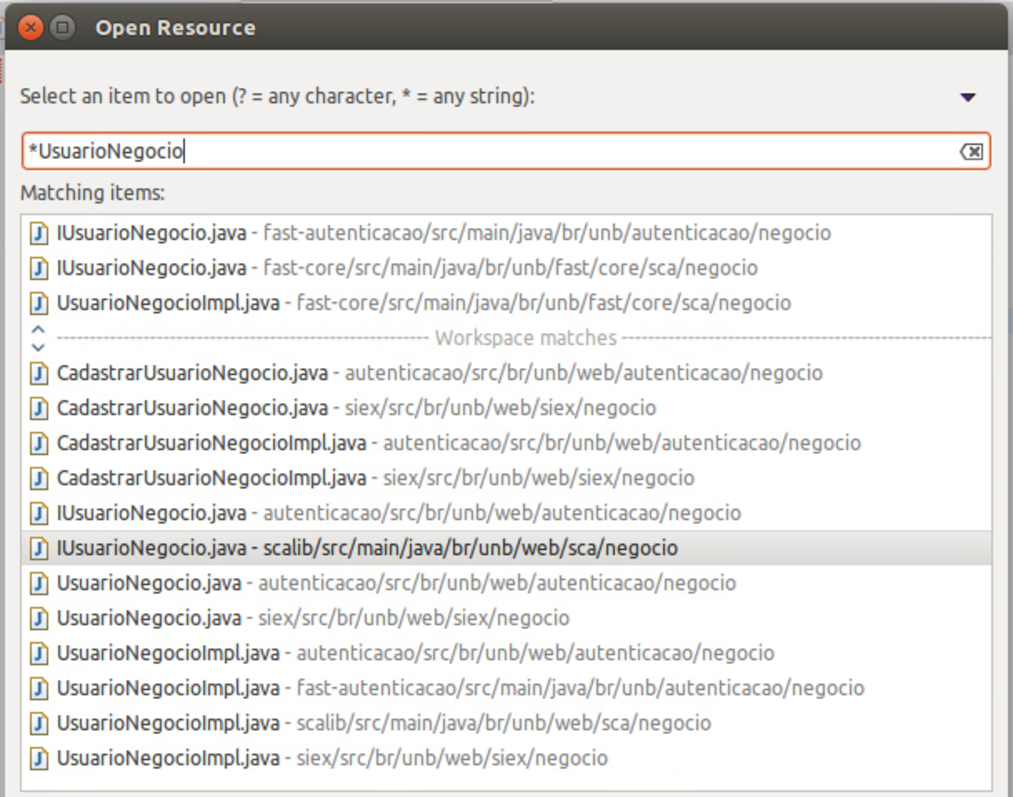
\includegraphics[scale=0.8]{img/avaliacao/QP2/duplicidade_usuario_negocio.pdf}
\caption{Exemplo de classe duplicada entre os sistemas Java.}
\label{fig:duplicidade_usuario_negocio}
\end{figure}

De acordo com o exposto, percebe-se que a manutenibilidade dos sistemas legados da Universidade
(como o \acrshort{SAE} legado) e mesmo os sistemas migrados para Java a partir de 2010,
foram muito impactados pela ausência de modularidade, integração e um bom design arquitetural, tendo como alguns efeitos colaterais observados já discutidos, a duplicidade das regras de negócios, a falta de reuso, a complexidade dos sistemas e o alto custo de manutenção. Assim, possivelmente, uma abordagem SOA aliada a uma boa arquitetura para o desenvolvimento dos serviços poderia minimizar tais problemas.

Nesse aspecto, o último diagrama da Figura~\ref{fig:dependency_diagram_sae_java}, apresenta a arquitetura do novo \acrshort{SAE} usando a arquitetura da abordagem proposta. Uma das preocupações levantadas desde o início dos trabalhos foi a integração lógica das aplicações através de uma camada \acrshort{SOA}, sendo esse papel, realizado pelo barramento e pelo \acrshort{SDK} \emph{ems\_java}, que juntos forneceram uma plataforma \acrshort{SOA} aderente à arquitetura \emph{RESTful} para o projeto. Como é possível notar no diagrama, todos os módulos desenvolvidos na modernização podem compartilhar as suas funcionalidades de forma transparente, bastando invocar os serviços disponíveis no catálogo de serviços do barramento. Salienta-se que o design interno dos módulos auxiliou muito para se chegar nesse objetivo. 

Assim, como discutido na QP1, uma das preocupações dos participantes do estudo de caso foi
empregar um design menos procedimental, razão pela qual decidiu-se utilizar o design \acrshort{DDD}. Este design provê algumas práticas que auxiliam o desenvolvimento de softwares~\cite{evans2004domain}. Uma dessas práticas é a modelagem de domínio do negócio, que promove uma abstração do domínio por meio de um modelo que contempla os aspectos relevantes ao desenvolvimento das aplicações, separando os interesses em domínios de negócios (ou domínios de contextos) separados. Este padrão sugere ainda uma estrutura de objetos que permite que o modelo seja implementado e refletido no código fonte por meio de uma linguagem comum entre as pessoas envolvidas no projeto, seja o especialista no domínio do negócio ou o desenvolvedor~\cite{evans2004domain,vernon2013implementing}. Entre as vantagens indicadas por~\cite{evans2004domain}, está a possibilidade de se obter mais proveito dos benefícios da orientação a objetos, tornando a arquitetura da aplicação mais flexível, fácil de manter e evoluir
com o passar do tempo. 

Nesse sentido, para exemplificar, a Figura~\ref{fig:exemplo_ddd} mostra um exemplo de uma classe Aluno do novo \acrshort{SAE} usando os princípios do \acrshort{DDD}. Foi removido alguns trechos do código fonte original de modo a facilitar a visualização. Como pode-se notar, a classe Aluno possui algumas responsabilidades manifestadas nos métodos declarados nessa classe. Caso fosse utilizado o padrão \textit{Transaction Script}, esta classe não teria nenhum método (objetos anêmicos) e possivelmente as responsabilidades estariam em uma classe de negócio com a classe Aluno servindo meramente como uma estrutura para passar os dados de um aluno entre as camadas do software até a camada de persistência.

\lstset{language=Java,
  basicstyle=\small, %or \small or \footnotesize etc.
  numbersep=10pt,                         % how far the line-numbers are from the code
  tabsize=4,  
  showspaces=false,
  showtabs=false,
  breaklines=true,
  showstringspaces=false,
  breakatwhitespace=true,
  commentstyle=\color{pgreen},
  keywordstyle=\color{pblue},
  stringstyle=\color{pred},
  captionpos=b,
  inputencoding=utf8,
  extendedchars=true,
  literate={á}{{\'a}}1 {ã}{{\~a}}1 {é}{{\'e}}1 {ê}{{\^e}}1 {ç}{{\c{c}}}1 {Ç}{{\c{C}}}1
}
\renewcommand{\lstlistingname}{Código}
\begin{lstlisting}[caption=Exemplo da classe Aluno do sistema SAE, label=fig:exemplo_ddd]
package br.unb.model.sae_context;

public class Aluno {
	private List<OcorrenciaAluno> listaOcorrenciaAluno;

	public void adicionaOcorrenciaAluno(OcorrenciaAluno ocorr){
		if (existeOcorrenciaAberto(ocorr.getSemestreAno(), ocorr.getDataInicio())){
			throw new Exception("O aluno já possui uma ocorrência.");
		}
		
		if (assinouTermoOcorrencia(ocorr.getSemestreAno())){
			throw new Exception("O aluno não possui termo de concessão assinado.");
		}
		
		listaOcorrenciaAluno.add(ocorr);
	}
	
	public List<OcorrenciaAluno> getListaOcorrenciaAluno() {
		return listaOcorrenciaAluno;
	}

	public boolean existeOcorrenciaAberto(String semestreAno, Date dataInicio){
		// Removido para melhor visualização
	}
	
	public boolean assinouTermoOcorrenciaValeAlimentacao(String semestreAno){
		// Removido para melhor visualização
	}
}
\end{lstlisting}





Finalizando a análise da questão QP2, verificaram-se alguns indicativos
qualitativos discutidos que sugerem que a manutenibilidade poderia ser maximizada tanto
pelo processo simplificado da abordagem quanto pela arquitetura
proposta. Porém, alguns desafios identificados durante o estudo de caso
ainda precisam ser melhor investigados para que a abordagem possa ser utilizada. Os 
principais desafios são descritos a seguir:

\begin{itemize}

	\item \textbf{Identificar os serviços que falharam.} A tolerância a falhas não foi o foco deste trabalho mas deverá ser investigado futuramente caso o \acrshort{CPD} opte pela abordagem. Durante os testes, verificou-se que não era possível mapear qual serviço de fato era a origem da falha. Isso pode ser um problema da arquitetura implementada. Por exemplo, quando se introduzia uma falha em um serviço (como o serviço de questionário), vários outros serviços deixavam de funcionar e não era possível identificar que serviço realmente falhou (o que é importante para poder corrigí-lo rapidamente). Seria importante a arquitetura permitir visualizar (se possível) a pilha de chamadas entre os serviços, para verificar qual serviço falhou. Sabe-se que uma das restrições que 
o estilo arquitetural \acrshort{REST} estabelece é que a interação entre 
o cliente e o servidor não deve manter estados entre as comunicações~\cite{fielding2000architectural}. No entanto, a arquitetura da plataforma permite que os serviços comuniquem-se internamente no \textit{cluster} de forma transparente, uma vez que cada serviço é na verdade um processo\footnote{Se o serviço for em Erlang é um processo do ambiente de execução Erlang e, se for em Java é uma \textit{thread} da máquina virtual Java.} que envia/recebe mensagens assíncronas Erlang. Nesse caso, quando um cliente envia uma \emph{requisição REST} para o barramento de serviços e este repassa para o seu destino (o serviço solicitado), a partir daí, as chamadas para outros serviços 
no \textit{cluster} são mensagens Erlang, sendo que nesse caso, poderia haver uma forma de identificar a sequência de chamadas entre os serviços internos para atender a solicitação do cliente, uma vez que todas as chamadas entre os processos passam primeiro pelo processo \emph{Dispatcher} do barramento. 

	\item \textbf{Transformar código procedimental em serviço.}

Este desafio está relacionado as atividades de análise e surgiu devido a dificuldade inerente para transformar código procedural em serviços durante a modernização do \acrshort{SAE}. Note que essa foi uma das atividades identificadas na QP1 mais difíceis de serem realizadas. Em um processo de modernização típico do CPD, que atualmente não é documentado, a migração dos sistemas legados segue o conceito \textit{Transaction Script}, que é relativamente mais direta e fácil de se fazer, uma vez que simplesmente se reescreve o que está no sistema legado para o novo sistema. Não é necessário pensar muito em como fazer, no máximo, vai haver a separação dos códigos de negócios da interface com o usuário e será criado a camada de persistência. Por outro lado, quando se pensa em oferecer serviços reutilizáveis, é necessário pensar na forma como será exposto o serviço, quais os parâmetros de entrada e o que o serviço vai retornar, para que ao final, tenha um bom design da \acrshort{API} e possa ser utilizado pelos clientes.

\end{itemize}


% Diagrama de dependências das três versões do SAE
%======================================================================================


\begin{figure}[htb]
\centering
\includegraphics[scale=0.37]{/img/avaliacao/QP2/metrics/SaeVB/ComponentDependenciesDiagram.png}
\caption{Diagrama de dependências do sistema \acrshort{SAE} na versão VB.}
\label{fig:dependency_diagram_sae_vb}
\end{figure}



\begin{figure}[htb]
\centering
\includegraphics[scale=0.37]{/img/avaliacao/QP2/metrics/SaeWeb/ComponentDependenciesDiagram.png}
\caption{Diagrama de dependências do sistema \acrshort{SAE} na versão C\#.}
\label{fig:dependency_diagram_sae_csharp}
\end{figure}



\begin{figure}[htb]
\centering
\includegraphics[scale=0.4]{/img/avaliacao/QP2/metrics/SaeJava/ComponentDependenciesDiagram.png}
\caption{Diagrama de dependências do sistema \acrshort{SAE} na versão Java.}
\label{fig:dependency_diagram_sae_java}
\end{figure}


\subsection{An\'{a}lise Relacionada à Terceira Questão de Pesquisa}

\begin{enumerate}[(QP3)]

\item Quais as razões que levam as organizações a modernizarem os seus sistemas legados?

\end{enumerate}

De acordo com as publicações analisadas, observa-se que, de maneira geral, existem 5 razões para um projeto de modernização dos sistemas legados, conforme descrito a seguir: 

\begin{itemize}

\item \textbf{Falta de integração entre os sistemas --} É cada vez maior a demanda por sistemas integrados nas 
organizações para prover a automação dos processos de negócio e permitir uma gestão com maior racionamento de recursos. 
Contudo, de acordo com~\cite{S3_Bisbal:1999, S29_Chung:2007, S31_LiuYan:2008}, muitos sistemas legados não foram projetados 
para serem integrados, razão pela qual as organizações investem em projetos de modernização, visando a integração dos fluxos e 
compartilhamento das funcionalidades de negócio existentes. Conforme 
observado em~\cite{S4_bennett1995legacy, S15_Comella-DordaASurvey2000, S2_erlikh:2000, Umar:2009}, 
existem vários outros benefícios obtidos com a integração dos sistemas tais como, a diminuição da quantidade de implementa\c c\~{o}es de regras 
de neg\'{o}cio duplicadas, a reutilização de soluções de software já desenvolvidas e a 
diminuição dos custos com o desenvolvimento.

\item \textbf{Tornarem-se mais flexíveis a mudanças --} Uma das principais razões que levam as organizações a buscarem a modernização 
dos seus sistemas legados é para torná-los mais flexíveis 
a mudanças~\cite{S4_bennett1995legacy, S01_bennett2000software, S3_Bisbal:1999, S15_Comella-DordaASurvey2000, S13_ransom1998method, 
S12_WeidermanApproaches:1997}. 
Para Bennet~\cite{S4_bennett1995legacy}, o \textit{time-to-market} dos sistemas é prioridade número 1 para a maioria das organizações. 
Em~\cite{S3_Bisbal:1999, S4_bennett1995legacy}, é relatado que muitos sistemas começam a ser chamados de sistemas legados, justamente porque 
passam a resistir mais as modificações que devem ser feitas, o que dificulta as evoluções no software que precisam ser implementadas para os negócios das organizações. 
Este pensamento vai de acordo com o que diz~\cite{S2_erlikh:2000}: ``A maioria das empresas querem transformar suas aplicações para atender a novos negócios e demandas, 
mas porque os sistemas legados tendem a ser de difícil controle, monolíticos e inflexíveis, muitas empresas consideram a modernização como em algum lugar entre improvável e impossível''. 

\item \textbf{Minimizar o custo de manutenção com o legado --} Reduzir o custo de manutenção dos sistemas legados é um dos grandes desafios para as organizações. 
Para~\cite{S4_bennett1995legacy, S15_Comella-DordaASurvey2000, S13_ransom1998method, S12_WeidermanApproaches:1997}, os 
sistemas legados são sistemas usualmente críticos para os negócios mas que o custo dispendido para mantê-los funcionando é quase sempre injustificável. 
\cite{S10_canfora2000decomposing} enfatiza que a manutenção frequentemente monopoliza os esforços das organizações, pois tais atividades, 
incluindo correção de erros, adaptações e melhorias em geral, consomem entre 50\% e 70\% do orçamento de um software típico. 
Adicionalmente,~\cite{S3_Bisbal:1999, S13_wu1997butterfly:1997} destacam que a falta de documentação e do conhecimento interno dos sistemas é um 
dos motivos dos altos custos bem como da demora nas manutenções para correção de falhas nos softwares. Portanto, como afirma~\cite{S4_bennett1995legacy}, há um dilema: 
de um lado, o sistema é muito valioso e uma substituição pode ser muito cara para ser contemplada. E, por outro lado, o sistema torna-se muito caro para manter e a
s demandas das organizações podem não ser sustentadas. Além do mais,~\cite{S23_warren2002renaissance} enfatiza que 
a substituição de um sistema legado poderia incorrer no risco da perda de informações críticas do negócio da organização.

\item \textbf{Falta de conhecimento e domínio do legado --} Como mencionado anteriormente, a falta de conhecimento e domínio nos sistemas legados 
é uma das justificativas para um projeto de modernização. De acordo com~\cite{S4_bennett1995legacy, S3_Bisbal:1999}, o entendimento 
do funcionamento de um sistema é visto como um dos requisitos para fazer as modificações que são requeridas pelas organizações. Tem sido reportado na 
literatura que uma parte substancial do tempo envolvido na compreensão de um sistema legado é na localização dos conceitos de domínio do problema a ser 
resolvido no código fonte para então serem feitas as implementações~\cite{S4_bennett1995legacy, clements2002documenting}. Assim, a compreensão dos sistemas legados representa 
um dos problemas de pesquisa centrais da literatura, conforme salienta~\cite{S4_bennett1995legacy}. 
Muitas pesquisas são despendidas para identificar
formas de obter um melhor entendimento do sistema que é vital para qualquer 
exercício de evolução como sugere~\cite{S01_bennett2000software, S13_ransom1998method}. Além 
disso,~\cite{S4_bennett1995legacy} reitera que existem os problemas de gerenciamento de pessoal. A maioria dos engenheiros de software preferem trabalhar em 
novos sistemas em vez de manter sistemas antigos e de tecnologia ultrapassada. E \textit{skills} necessários podem estar cada vez mais reduzidos e escassos, decorrente da saída dos profissionais que conhecem esses sistemas das organizações.

\item \textbf{Propenso a falhas --} De acordo com~\cite{S4_bennett1995legacy}, sem documentação atualizada, as evoluções nos softwares são efetuadas usando 
o próprio código fonte como documentação confiável. Aliado aos problemas de gerenciamento de pessoal, acredita-se que os sistemas podem ser alvo de 
falhas pela falta de conhecimento e domínio nesses sistemas. Apesar disso,~\cite{S4_bennett1995legacy} afirma que os sistemas podem ser muito confiáveis e 
responsivos para as necessidades dos usuários, bem mais do que um novo sistema que viesse a substituir o atual. No entanto, existe um sentimento percebido por várias organizações que os sistemas legados podem falhar devido a falta de especialistas e/ou suporte (empresas que mantêm e dão treinamento em tecnologias legadas). Nesse sentido, uma falha poderia causar um sério impacto para as organizações, como afirma~\cite{S3_Bisbal:1999}.

\end{itemize}



\section{Síntese do Capítulo}

As organizações querem 
adaptar-se rapidamente as mudanças nos requerimentos de negócios,
sejam elas intra-organizacionais, alterações em leis ou 
regulamentações; mudanças que envolvem 
a modernização dos sistemas legados e a
atualização de tecnologias.

Como visto neste capítulo, 
independente do ciclo de vida selecionado para
descrever a evolução de um sistema legado, 
de acordo com~\cite{S3_Bisbal:1999,S12_WeidermanApproaches:1997}, 
determinar qual é a atividade mais apropriada
em diferentes pontos pode ser um grande desafio: devemos
continuar mantendo o sistema, modernizá-lo ou substituí-lo?
Ao tomar esta decisão, as organizações devem avaliar seus
sistemas legados, de modo que se possa 
determinar a melhor estratégia de evolução e
identificar as implicações de cada ação~\cite{Seacord:2003}. 

Nesse contexto, foi muito importante compreender
as estratégias de modernização dos sistemas legados descritos na literatura.
Após este \acrfull{MS}, tornou-se claro que um processo de 
modernização com uma abordagem sistemática deveria ser proposto ao CPD/UnB,
para diminuir os custos e os riscos associados com a 
modernização dos sistemas legados, ao permitir continuar mantendo
os sistemas atuais enquanto a migração acontece em paralelo
de forma gradativa.
